\documentclass[a4paper,11pt] {article}
% Default margins are too wide all the way around. I reset them here
\setlength{\topmargin}{.5in}
\setlength{\textheight}{9in}
\setlength{\oddsidemargin}{.125in}
\setlength{\textwidth}{6.25in}

\usepackage{color}
\usepackage[utf8]{inputenc}
\usepackage{graphicx}
\usepackage{float}
\usepackage{pdfpages}
\usepackage{amsthm}
\usepackage{amsmath,amsfonts,amssymb,amsthm}
\theoremstyle{definition}
\newtheorem{defn}{Definition}[section]
\newtheorem{conj}{Conjecture}[section]
\newtheorem{exmp}{Example}[section]

\definecolor{javared}{rgb}{0.6,0,0} % for strings
\definecolor{javagreen}{rgb}{0.25,0.5,0.35} % comments
\definecolor{javapurple}{rgb}{0.5,0,0.35} % keywords
\definecolor{javadocblue}{rgb}{0.25,0.35,0.75} % javadoc
%\usepackage[french]{babel}
\usepackage[T1]{fontenc}


\begin{document}
\title{\textbf{Usability and Skeuomorphism}}
\author{\textbf{Bodart Xavier} - \textbf{Chapeaux Thomas} - \textbf{Mayeur Bernard} \\
Université Libre de Bruxelles}

\maketitle
\begin{center}

\textbf{INFO-F501 Information technology in society} \\
Luc WILKIN
\end{center}
\begin{center}

~\\


\includegraphics[scale=0.15]{fig-report/ULBjea.jpg}
\end{center}
\pagebreak
\tableofcontents
\pagebreak
\section{Introduction}

Most tools we use today, from wristwatches and squirt guns to smartphones and industrial softwares, rely on sophisticated technology hidden from the user. This require the user to be taught how to use the tool, which can be done with manuals and trial-and-error, but also by designing the tool in such a way that its usage is both obvious and simple.\\

While this has been done for centuries for physical objects using switches, knobs and buttons, the most recent computing devices tends to have a simplistic physical design (often reduced to a black surface with a touchscreen) and use abstract elements on the screen to interact with the user by touch, leaving the responsibility of design to the application creator.\\

In this document, we concentrate on design trends in electronic tablet applications. In Sect.~\ref{sct:theory}, we present some of the basic design principles described in [CITATION NEEDED] which can be applied to the design of any object.\\

Then, in Sect.~\ref{sct:history}, we show how those principles can be recognized in the evolution of the design of computer systems, concluding with the current trends in electronic tablets, namely skeuomorphism and flat design.\\

Finally, in Sect.~\ref{sct:experiment}, we present experimentation results demonstrating how users react to those designs. One result is from our own experiment, in which we confronted various users to a skeuomorphic calculator application and to a flat one.\\

\section{Theoretical concepts and design principles}
\label{sct:theory}

    \subsection{Perceived affordance}

Perceived affordance represents the quality of an object to suggest its utilization. This concept is quite important in object-design due to the fact that it may represents the main source of information about the usage of the object. Indeed, people tends to read less and less the usage notice. In addition, this concept may reinforce the feeling of experience of a person for a given object.

\begin{figure}[h]
\centering
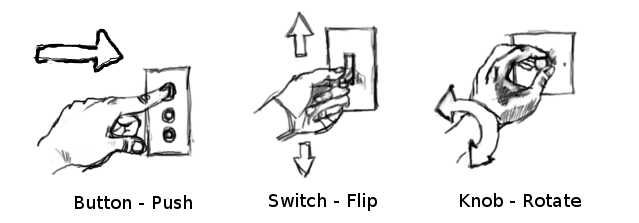
\includegraphics[scale=0.40]{fig-report/switches-only.png}
\caption{By their forms, buttons,switches or knobs often suggest their working.}
\end{figure}

Perceived affordance is not always the same as real affordance. Indeed, design can rarely explain the complete working of complex objects. The perceived affordance is only capable of showing primitive properties of its usage. Furthermore, a bad design may induce an usage more difficult than the correct design\cite{affordancesMads}.

\begin{figure}[h]
\centering
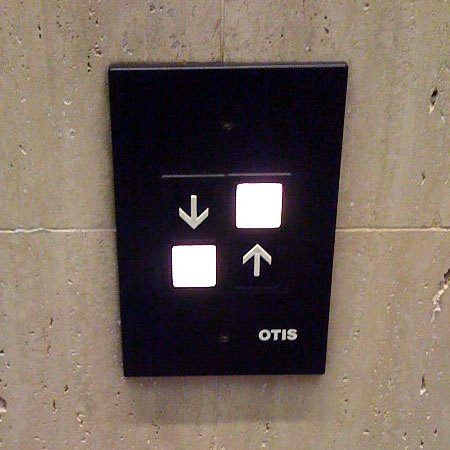
\includegraphics[scale=0.20]{fig-report/bad-switches.jpg}
\caption{What would you do in front of such a lift panel?}
\end{figure}

    \subsection{Natural mapping}
Natural mapping is the concept of organizing controllers in the same arrangement as the objects on which they have an influence to guarantee the expected result. This principle will often lead to an increase in perceived affordance.\\

A common example to illustrate this concept is the placement of the buttons that control the different stoves of your kitchen.It's obvious that the most left-top button will regulate the temperature of the most left-top stove.\\
 \begin{minipage}{\linewidth}
      \centering
      \begin{minipage}{0.45\linewidth}
          \begin{figure}[H]
          \centering
              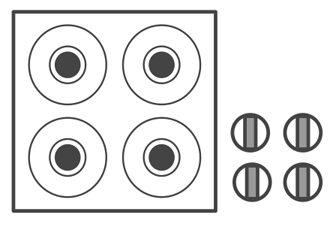
\includegraphics[scale=0.3]{fig-report/stove_natural.png}
              \caption{Scheme of a four stoves set with their corresponding knobs}
          \end{figure}
      \end{minipage}
      \hspace{0.05\linewidth}
      \begin{minipage}{0.45\linewidth}
          \begin{figure}[H]
                    \centering
              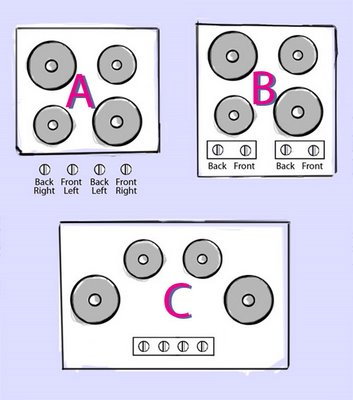
\includegraphics[scale=0.4]{fig-report/NormanBurners.jpg}
              \caption{These designs work only if you have the same assumption as the designer\cite{stoveMapping}}
          \end{figure}
      \end{minipage}
  \end{minipage}
  \bigskip


Unfortunately, this principle may sometimes induce extra design cost and may also depends on the point of view of the designer: Even if it seems logical for certain arrangement such stoves or the control of the electronic windows of the car, One can still doubt about the mapping of light switches(\textit{"Does this switch controls  the lights of the front of the room because it is above the others ?"}).

    \subsection{Feedback}
\newtheorem{mydef}{Definition}
\begin{mydef}
\textit{\textbf{Feedback}}: sending back to the user information about what action has actually been done, what result has been accomplished.
\cite{Norman02}
\end{mydef}

In our case, feedback represents any action that could indicate to the user that its interaction with the item was taken into account. In certain cases, feedback can be done implicitly by the quality and the design of the object itself. For example, when a push button is  pressed, one can hear a clicking sound. On the other hand, feedback often requires, in our modern technologies, additional functions like vibrating or emitting sounds that corresponds to states of the device. Theses retro-actions have to provide enough information to the user in order to avoid his frustration about a mistaken usage.

\begin{figure}[h]
\centering
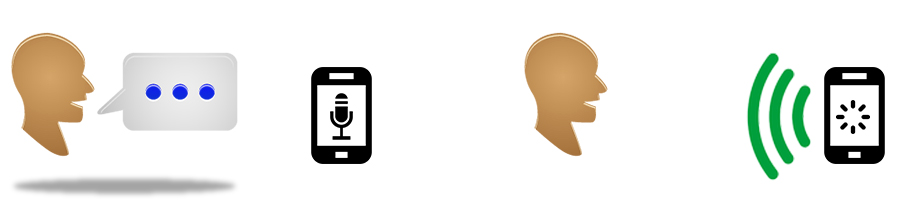
\includegraphics[scale=0.5]{fig-report/retro-action-speaking.jpg}
\caption{After the user gives a command, the device emits a sound to confirm that it is analyzing the request}
\end{figure}

    \subsection{Additional design principles}

As presented in \cite{Norman02}
, one can also add two principles to a good design:
\begin{itemize}
\item \textbf{Provide a good conceptual model}: The idea is to provide a precise information model about the good usage of the item, or the way to maintain it. Written instructions should guarantee the good usage of the item. The design of such scheme is really important and should be extremely clear.
\item \textbf{Make things visible}: Certain of our modern items can be seen as real complex state machines due to the number of actions they can propose. The basic idea behind this principle is to provide a display which shows the current state and the available actions. A good example to this is the usage of a new VoIP telephone which allow a user to start a conference with several other people. Such telephone are often equipped with a large display which can show different contacts number, propose features to start conference or even to place a call on hold in order to answer to another call.
\end{itemize}

 \begin{minipage}{\linewidth}
      \centering
      \begin{minipage}{0.45\linewidth}
          \begin{figure}[H]
          \centering
              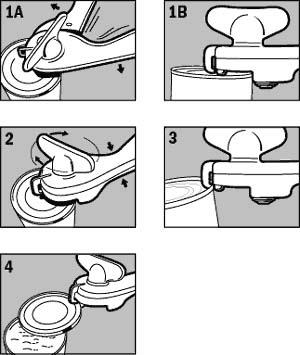
\includegraphics[scale=0.4]{fig-report/can-opener}
              \caption{Does such model give enough information about the usage of a can-opener ?}
          \end{figure}
      \end{minipage}
      \hspace{0.05\linewidth}
      \begin{minipage}{0.45\linewidth}
          \begin{figure}[H]
                    \centering
               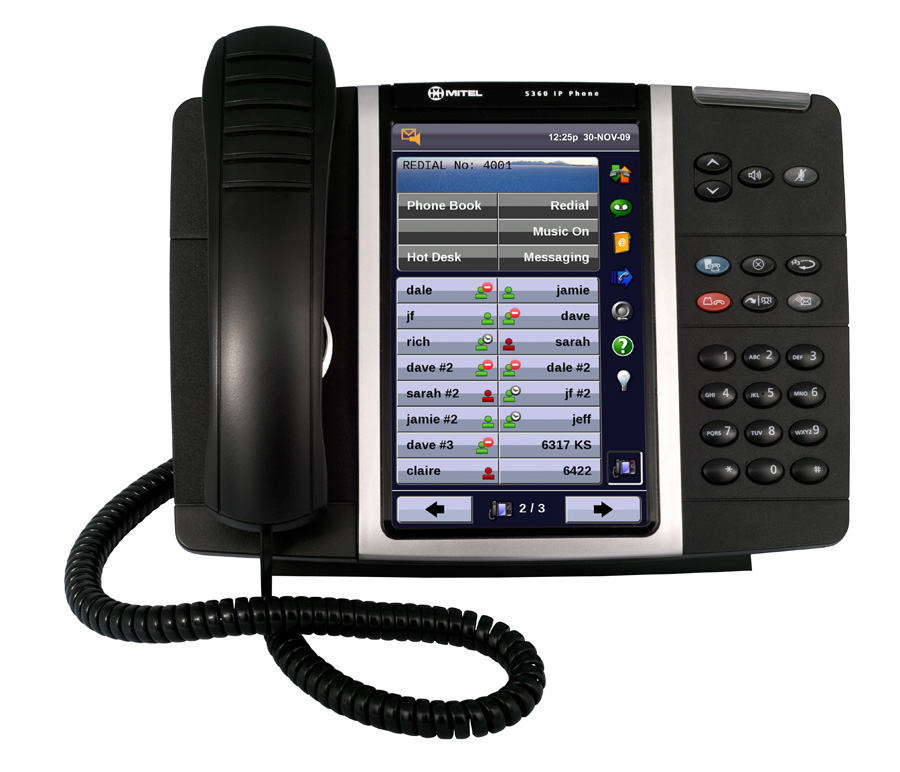
\includegraphics[scale=0.7]{fig-report/voip-phone.jpg}
              \caption{This VoIP phone has a big display to propose multiple commands}
          \end{figure}
      \end{minipage}
  \end{minipage}

    \subsection{Constraints}
	In addition with affordances, usage of objects is also induced by natural constraints such as physical constraints, logical constraints, cultural constraints, \ldots. These implicit rules may depend on the knowledge of the user but might increase perceived affordance. In the following subsections, each type of constraints will be explained and illustrated with an example.
        \subsubsection{Physical constraints}
        These constraints are the strongest ones because they reduce considerably the number of possible 	usages: Even without any attempt, the user will often be able to obviously discard  alternatives. They do not or poorly depend on the knowledge of the user.\\

        $\underline{Example:}$\\
        When a builder has just finished his work, he has to refill his toolbox which contains dedicated 		slots. It's completely impossible for him to put his hammer into the slot initially defined for a screwdriver.
        \begin{figure}[h]
        \centering
        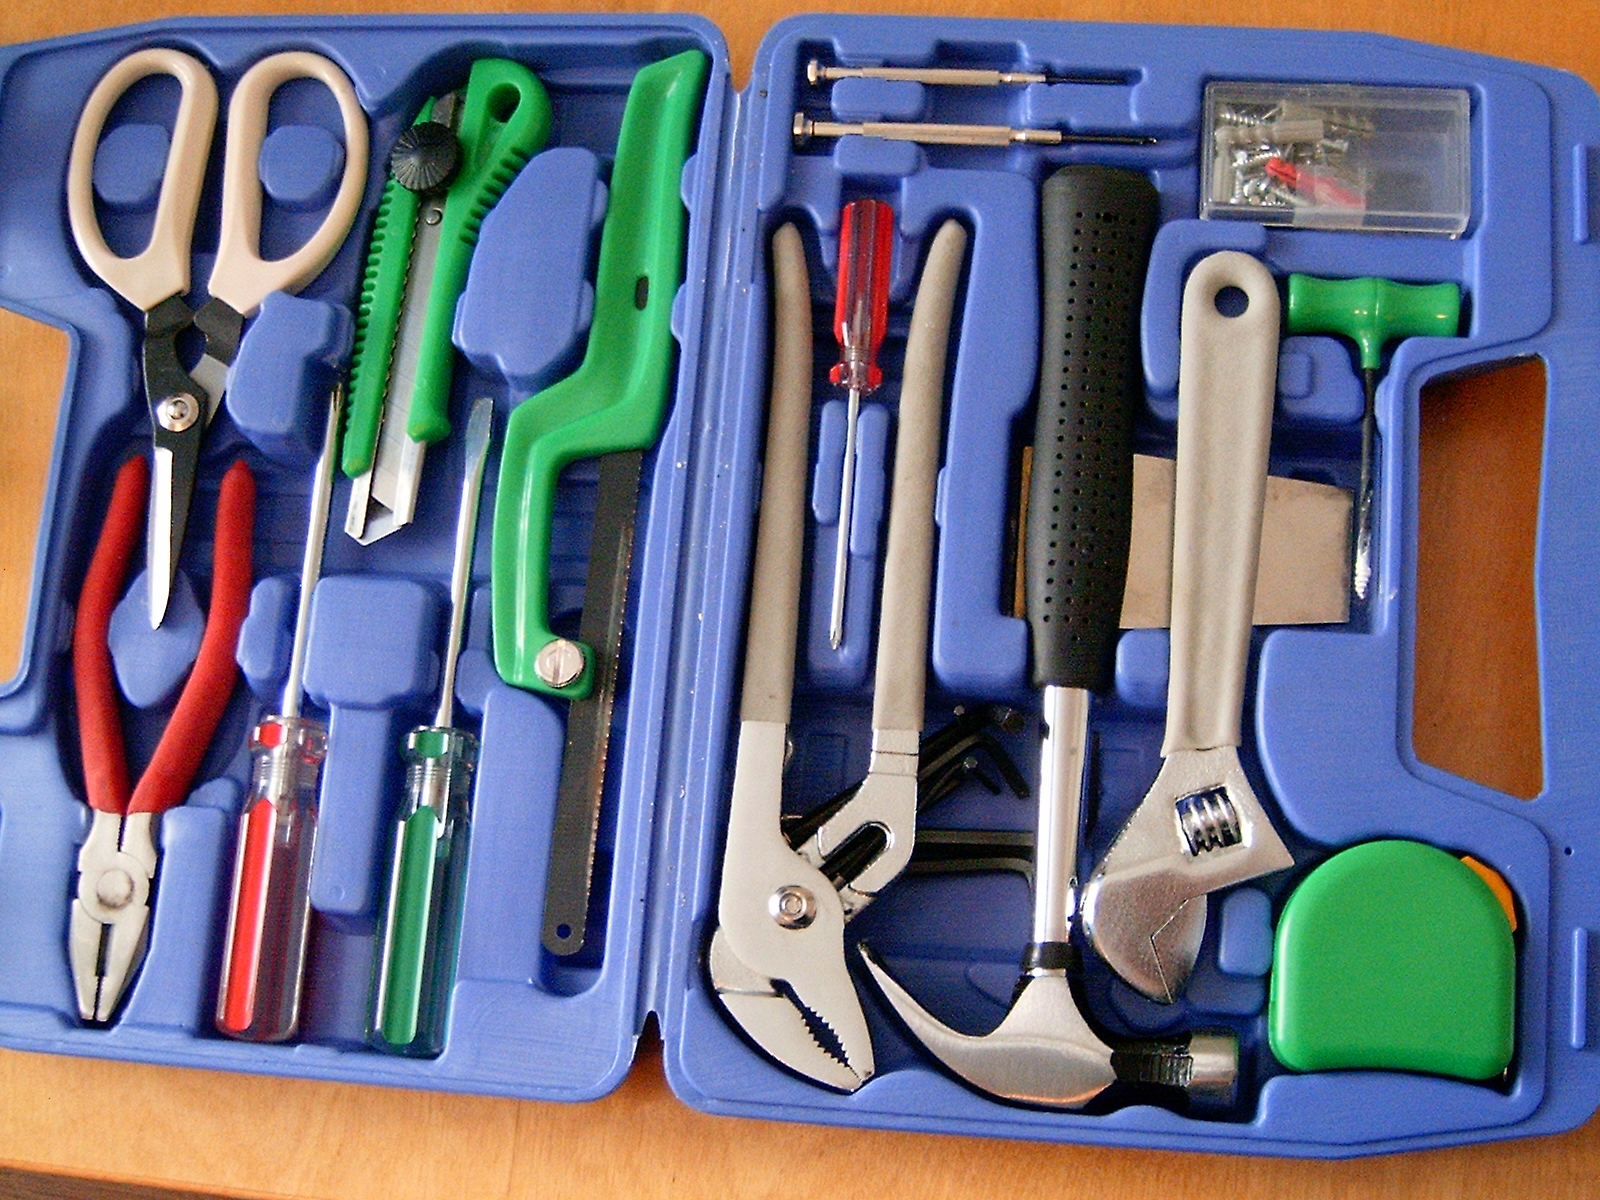
\includegraphics[scale=0.1]{fig-report/toolbox.jpg}
        \end{figure}
        \subsubsection{Semantic constraints}
       In opposition to the physical constraints, semantic constraints require a good knowledge about the situation in which the object should be used.\\

        $\underline{Example:}$\\
        A simple example is shoe laces. It's difficult for a novice to do it correctly the first time. After a while, such actions will appear simple and logical.
        \begin{figure}[h]
        \centering
        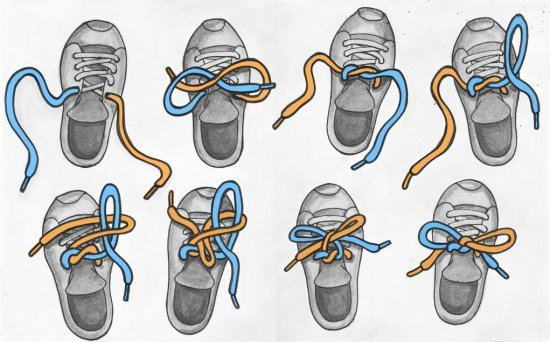
\includegraphics[scale=0.3]{fig-report/tie_your_shoes.jpg}
        \end{figure}
        \subsubsection{Cultural constraints}
        These constraints are the consequences of cultural conventions which have existed for several years. These constraints can be considered arbitrary because in most of the cases, several possible alternatives could be applicable. Indeed such constraints do not affect the semantic or the physical usage of the given object. Unfortunately, these constraints may change depending on the the geographical and temporal context. Furthermore, problems could arise when such constraints have to be decided for new items\\

        $\underline{Example:}$\\
        A basic example could be the disposition and the color of the traffic lights. In western countries, the green color represents the fact that you can go on and traffic lights are positioned in a vertical column . In opposition, in Japan, traffic lights may be composed of blue, orange and red lights, and could be displayed as a horizontal row.
        \begin{figure}[h]
        \centering
        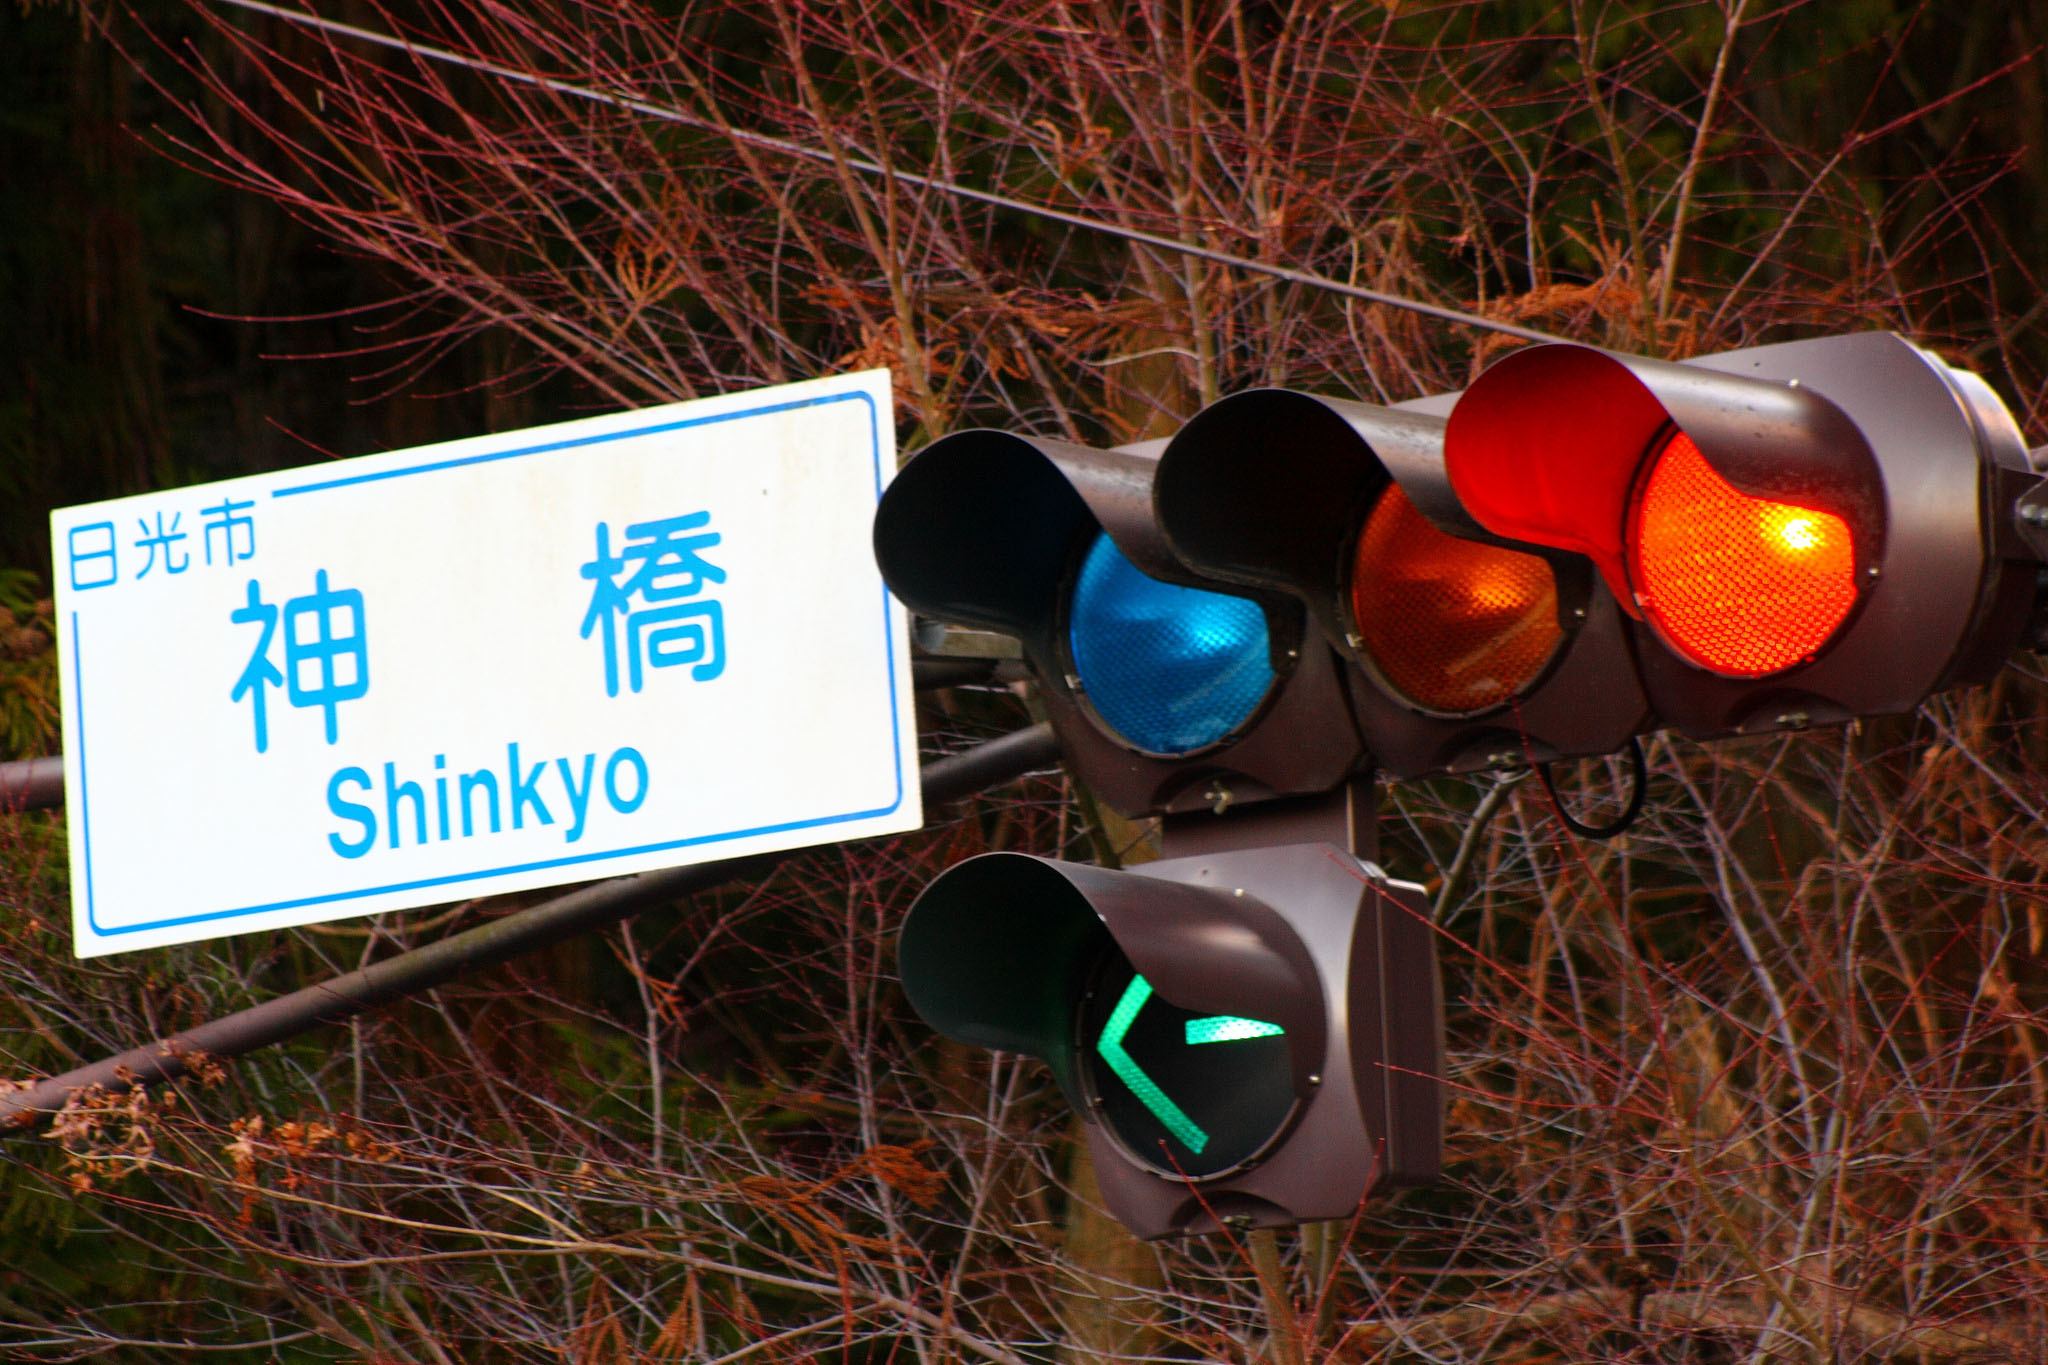
\includegraphics[scale=0.1]{fig-report/japan-traffic-light.jpg}
        \end{figure}

        \subsubsection{Logical constraints}
        These constraints call to the good-sense of the user. No physical or cultural knowledge is required here. The only thing that matters here is to confirm the first and logical assumption of user through design choices. Such constraints are often linked to natural mapping.\\

        $\underline{Example:}$\\
        The most trivial example could be the fact that a left switch will always activate the leftmost light.




\section{Evolution of the computer-interface}
\label{sct:history}

    \subsection{Command line interpreter}
    \subsection{Graphical interface and computer mouse}
    \subsection{Touch interface}
    \subsection{Voice interface}
    \subsection{Neural interface}
    \subsection{Current trends in touch interface}
        \subsubsection{Skeuomorphism}
        \subsubsection{Flat design}


\section{Experiment}
\label{sct:experiment}

    \subsection{Definition of the experiment}
    \subsection{Results analysis}
    \subsection{Comparison with previous studies}

\section{Conclusion}
\bibliographystyle{plain}
\bibliography{bibUsability}
\end{document}
